\documentclass[11pt]{article}

% --- Packages ---
\usepackage[utf8]{inputenc}
\usepackage[T1]{fontenc}
\usepackage{amsmath,amssymb}
\usepackage{booktabs}
\usepackage{graphicx}
\usepackage{hyperref}
\usepackage{xcolor}
\usepackage{natbib}
\usepackage{microtype}
\usepackage{float}
\usepackage{enumitem}
\usepackage{multirow}
\usepackage[margin=1in]{geometry}
\usepackage{caption}
\usepackage{subcaption}
\usepackage{url}
\usepackage{algorithm}
\usepackage{algorithmic}

\hypersetup{
    colorlinks=true,
    linkcolor=blue,
    citecolor=blue,
    urlcolor=blue
}

% --- Title ---
\title{LLM-as-Researcher: Comparative Analysis of AI Models\\for Autonomous Neural Network Training Optimization}

\author{
    Patrick Hughes\\
    BMD PAT LLC\\
    \texttt{pat@bmdpat.com}
}

\date{March 23, 2026}

\begin{document}

\maketitle

% --- Abstract ---
\begin{abstract}
We evaluate large language models as autonomous ML researchers using the \texttt{autoresearch} framework \citep{karpathy2026autoresearch}. Each model iteratively proposes modifications to a 50M-parameter language model's training code, runs 5-minute experiments on PubMed medical abstracts, and keeps or reverts changes based on validation bits-per-byte (val\_bpb). In Phase 1 (exploratory), we sequentially ran Claude Sonnet 4, Claude Sonnet 4.6, and Claude Opus 4.6 (with 32K extended thinking), with each model building on previous improvements. Sonnet 4.6 achieved the highest keep rate (22.1\%) with the lowest crash rate (8.7\%), while Opus 4.6 found the deepest optimizations through multi-step causal reasoning. In Phase 2 (controlled, in progress), all models including GPT-4.1 start from an identical unoptimized baseline with $n=3$ runs per model, enabling direct statistical comparison. We provide detailed failure analysis, cost-effectiveness data, and practical guidance for researchers implementing similar pipelines.
\end{abstract}

% =============================================================================
\section{Introduction}
\label{sec:introduction}
% =============================================================================

Large language models have become standard coding assistants, but a more ambitious question remains open: can LLMs conduct research autonomously? Specifically, can they iteratively improve a machine learning training pipeline without human intervention, proposing hypotheses, running experiments, and learning from results?

Karpathy's \texttt{autoresearch} framework \citep{karpathy2026autoresearch} operationalizes this question. An LLM agent is given a training script, a dataset, and a single objective metric. It proposes code modifications as JSON patches, the framework applies them, trains for a fixed duration, evaluates validation performance, and keeps the change only if it improves the metric. Otherwise the change is reverted and the agent is informed of the failure. The agent receives the full experiment history and tries again.

This paper makes the following contributions:

\begin{enumerate}[leftmargin=*]
    \item \textbf{Multi-model comparison.} We run three LLMs through sequential experimental conditions in Phase 1 and compare keep rates, crash rates, cost-effectiveness, and the quality of discovered optimizations. Phase 2 adds GPT-4.1 in a controlled head-to-head design with $n=3$ replication.
    \item \textbf{Extended thinking analysis.} We demonstrate that Claude Opus 4.6 with 32K extended thinking tokens finds multi-step optimization chains that shorter-context models miss, particularly on already-optimized baselines.
    \item \textbf{Practical engineering insights.} We document Blackwell GPU (RTX 5070 Ti) compatibility issues, \texttt{torch.compile} failure modes, and cost planning guidance for researchers reproducing this work.
    \item \textbf{Open data.} We report full experiment logs including every proposed change, its outcome, and the resulting val\_bpb, enabling meta-analysis of LLM research strategies.
\end{enumerate}

% =============================================================================
\section{Related Work}
\label{sec:related}
% =============================================================================

\paragraph{Automated Machine Learning.}
AutoML \citep{hutter2019automl} encompasses hyperparameter optimization, neural architecture search (NAS) \citep{zoph2017nas}, and automated feature engineering. NAS methods typically define a fixed search space and use reinforcement learning or evolutionary algorithms to explore it. Our setting differs: the LLM operates on raw Python source code with no predefined search space, making the problem both harder (unbounded space) and more flexible (any valid code change is permitted).

\paragraph{LLM Code Generation.}
Codex \citep{chen2021codex} and AlphaCode demonstrated that LLMs can generate functionally correct programs from specifications. More recent models -- Claude Sonnet 4.6, Opus 4.6, and GPT-4.1 -- represent significant advances in code understanding and generation. However, generating code that \emph{improves} an existing training pipeline requires understanding not just syntax but the interactions between optimizer hyperparameters, model architecture, and training dynamics.

\paragraph{AI-Driven Scientific Discovery.}
The AI Scientist \citep{lu2024aiscientist} demonstrated end-to-end automated research including idea generation, experimentation, and paper writing. Our work is complementary but narrower in scope: we focus specifically on the optimization loop and use it as a controlled testbed for comparing LLM capabilities. Where The AI Scientist evaluates whether AI can do science, we evaluate which AI does it best.

\paragraph{The autoresearch Framework.}
Karpathy introduced \texttt{autoresearch} in early 2026 \citep{karpathy2026autoresearch} as an open-source tool for autonomous training optimization. The framework provides the agent loop, experiment logging, and keep/revert logic. Our work extends the framework with adaptive temperature scheduling, enhanced failure categorization, and multi-model support including Azure OpenAI endpoints.

% =============================================================================
\section{Methodology}
\label{sec:methodology}
% =============================================================================

% -----------------------------------------------------------------------------
\subsection{Framework}
\label{sec:framework}
% -----------------------------------------------------------------------------

The \texttt{autoresearch} loop proceeds as follows:

\begin{algorithm}[H]
\caption{Autoresearch Optimization Loop}
\label{alg:loop}
\begin{algorithmic}[1]
\STATE Initialize \texttt{train.py} with baseline configuration
\STATE Train baseline, record $\text{val\_bpb}_0$
\FOR{$i = 1$ to $N$}
    \STATE Send experiment history + current \texttt{train.py} to LLM
    \STATE LLM returns JSON patch (search/replace pairs)
    \STATE Apply patch to \texttt{train.py}
    \STATE Train for 5 minutes, record $\text{val\_bpb}_i$
    \IF{$\text{val\_bpb}_i < \text{val\_bpb}_{\text{best}}$}
        \STATE Keep change, update $\text{val\_bpb}_{\text{best}}$
    \ELSE
        \STATE Revert \texttt{train.py} to previous version
    \ENDIF
    \STATE Append result (kept/discarded/crashed) to history
\ENDFOR
\end{algorithmic}
\end{algorithm}

Several extensions were implemented for robustness:

\begin{itemize}[leftmargin=*]
    \item \textbf{Categorized history summaries.} The full experiment history is sent to the LLM each round, organized into kept, discarded, and crashed categories with near-miss highlighting for experiments that came close to improving.
    \item \textbf{Adaptive temperature.} For Sonnet models, the API temperature increases linearly from 0.0 to 0.5 during failure streaks, encouraging exploration when repeated proposals fail. Temperature resets to 0.0 after a successful keep.
    \item \textbf{FatalAPIError handling.} Billing failures, rate limits, and network errors are caught and retried with exponential backoff rather than counted as experiment failures.
    \item \textbf{Auto-restart.} \texttt{torch.compile} inductor bugs cause intermittent segfaults. The framework detects these and restarts the training process automatically.
\end{itemize}

% -----------------------------------------------------------------------------
\subsection{Model Architecture}
\label{sec:architecture}
% -----------------------------------------------------------------------------

The target model is a 50M-parameter decoder-only transformer, configured as shown in Table~\ref{tab:architecture}.

\begin{table}[H]
\centering
\caption{Baseline model architecture.}
\label{tab:architecture}
\begin{tabular}{ll}
\toprule
\textbf{Parameter} & \textbf{Value} \\
\midrule
Parameters & 50M \\
Layers & 8 \\
Attention heads & 4 \\
Embedding dimension & 512 \\
Optimizer & Muon + AdamW (embeddings) \\
Attention mechanism & SDPA \\
Compilation & \texttt{torch.compile} \\
Max sequence length & 2048 \\
\bottomrule
\end{tabular}
\end{table}

The Muon optimizer \citep{jordan2024muon} is used for all matrix-shaped parameters, while AdamW handles embedding parameters. Flash Attention 3 \citep{dao2024flashattention3} was unavailable on the Blackwell architecture at the time of experiments, so PyTorch's scaled dot-product attention (SDPA) was used as a fallback.

The use of \texttt{torch.compile} is important context for the experiment results: it constrains the space of valid code changes, since many architectural modifications break the compilation graph. This is a significant source of crashes, particularly for models with weaker code understanding.

% -----------------------------------------------------------------------------
\subsection{Dataset}
\label{sec:dataset}
% -----------------------------------------------------------------------------

All experiments use PubMed medical abstracts from the HuggingFace dataset \texttt{uiyunkim-hub/pubmed-abstract}, containing approximately 27.7 million abstracts. A BPE tokenizer with vocabulary size 8,192 was trained on the corpus. Maximum sequence length was set to 2,048 tokens.

PubMed abstracts were chosen for several reasons: the text is relatively homogeneous (structured medical writing), the dataset is large enough to avoid overfitting in 5-minute training runs, and the medical domain provides a practical testbed for language modeling on specialized technical text.

The evaluation metric is validation bits-per-byte (val\_bpb), which measures compression efficiency on held-out data. Lower values indicate better language modeling. This metric is preferred over perplexity because it is tokenizer-independent, enabling fair comparison across different vocabulary sizes if the tokenizer is modified.

% -----------------------------------------------------------------------------
\subsection{Hardware}
\label{sec:hardware}
% -----------------------------------------------------------------------------

All experiments were conducted on a single workstation:

\begin{itemize}[leftmargin=*]
    \item \textbf{GPU:} NVIDIA GeForce RTX 5070 Ti, 16GB VRAM, Blackwell architecture (SM 12.0)
    \item \textbf{OS:} WSL2 Ubuntu 22.04 on Windows 11 Pro
    \item \textbf{Software:} Python 3.12, PyTorch 2.9.1+cu128, CUDA 12.8
    \item \textbf{Thermal management:} Training pauses at 80\textdegree C GPU temperature, aborts at 90\textdegree C
\end{itemize}

The RTX 5070 Ti was among the first consumer Blackwell GPUs available and presented several compatibility challenges documented in Section~\ref{sec:blackwell}.

% -----------------------------------------------------------------------------
\subsection{LLM Configurations}
\label{sec:llm_configs}
% -----------------------------------------------------------------------------

Three LLM configurations were used in Phase 1, summarized in Table~\ref{tab:llm_configs}.

\begin{table}[H]
\centering
\caption{LLM configurations for each experimental run.}
\label{tab:llm_configs}
\begin{tabular}{lllllr}
\toprule
\textbf{Model} & \textbf{API} & \textbf{Thinking} & \textbf{Temperature} & \textbf{Timeout} & \textbf{Est.\ Cost/Exp} \\
\midrule
Claude Sonnet 4     & Anthropic     & None       & Adaptive (0--0.5)  & 180s  & \$0.06 \\
Claude Sonnet 4.6   & Anthropic     & None       & Adaptive (0--0.5)  & 180s  & \$0.06 \\
Claude Opus 4.6     & Anthropic     & 32K tokens & Fixed (1.0)        & 600s  & \$1--2 \\
\bottomrule
\end{tabular}
\end{table}

GPT-4.1 is evaluated in Phase 2 only (Section~\ref{sec:phase2}).

Opus 4.6 uses a fixed temperature of 1.0 as required by Anthropic's extended thinking API. The 32K thinking token budget allows the model to reason through multi-step optimization hypotheses before proposing changes. The substantially higher cost per experiment (\$1--2 vs.\ \$0.06) reflects the extended thinking token usage.

% =============================================================================
\section{Phase 1: Exploratory Sequential Optimization}
\label{sec:phase1}
% =============================================================================

In Phase 1, models were run sequentially, with each model's optimized code becoming the next model's starting baseline. This design was driven by practical constraints (overnight runs accumulating improvements), but it means improvement percentages are not directly comparable across models. Despite this limitation, Phase 1 provides valuable data about each model's optimization strategy and failure modes.

% -----------------------------------------------------------------------------
\subsection{Overall Comparison}
\label{sec:overall}
% -----------------------------------------------------------------------------

Table~\ref{tab:results} summarizes the performance of each model across all experiments.

\begin{table}[H]
\centering
\caption{Overall results for each LLM. Keep rate is computed over non-crashed experiments. Improvement is relative to each run's starting baseline.}
\label{tab:results}
\begin{tabular}{lrrrrrrr}
\toprule
\textbf{Model} & \textbf{Exps} & \textbf{Kept (\%)} & \textbf{Disc.} & \textbf{Crashed (\%)} & \textbf{Baseline} & \textbf{Best val\_bpb} & \textbf{Improv.\ (\%)} \\
\midrule
Sonnet 4     & 147 & 5 (5.2\%)   & 45 & 50 (34.0\%) & 0.9481 & 0.9362 & 1.25 \\
Sonnet 4.6   & 104 & 21 (22.1\%) & 70 & 9 (8.7\%)   & 1.2453 & 0.9559 & 23.24 \\
Opus 4.6     & 111 & 8 (8.9\%)  & 64 & 21 (18.9\%) & 0.9557 & 0.9019 & 5.64 \\
\bottomrule
\end{tabular}
\end{table}

\paragraph{Skipped experiments.} Not all experiments reached the training stage. When an LLM returned a response that could not be parsed as a valid JSON code patch, the experiment was skipped with no training run. Sonnet 4 had 47 such skipped experiments (32\% of total), Sonnet 4.6 had 4 (4\%), and Opus 4.6 had 18 (16\%). The skipped counts are included in the experiment totals but excluded from the kept/discarded/crashed breakdown. This metric is a practical measure of instruction-following reliability: Sonnet 4.6's near-zero skip rate reflects strong adherence to the required JSON output format, while Sonnet 4's high skip rate indicates frequent formatting failures that wasted experiment slots.

\textbf{Important caveat on baselines.} The three runs did not all start from the same baseline, which complicates direct comparison:

\begin{itemize}[leftmargin=*]
    \item \textbf{Sonnet 4} started from a partially optimized baseline (val\_bpb = 0.948) produced by earlier manual tuning.
    \item \textbf{Sonnet 4.6} started from the clean, unmodified master branch (val\_bpb = 1.245), giving it the most room for improvement.
    \item \textbf{Opus 4.6} started from Sonnet 4.6's best result (val\_bpb = 0.956), an already well-optimized configuration.
\end{itemize}

This sequential progression means that later models faced harder optimization landscapes. Opus 4.6's 5.64\% improvement on an already-optimized baseline is arguably more impressive than Sonnet 4.6's 23.24\% improvement from a cold start, though this claim is difficult to verify without controlled ablations.

% -----------------------------------------------------------------------------
\subsection{Key Discoveries by Model}
\label{sec:discoveries}
% -----------------------------------------------------------------------------

\subsubsection{Claude Sonnet 4}

Sonnet 4 found 5 improvements over 147 experiments. The successful changes were:

\begin{enumerate}[leftmargin=*]
    \item \textbf{Total batch size halving} (\texttt{TOTAL\_BATCH\_SIZE} from $2^{17}$ to $2^{16}$): More frequent gradient updates improved convergence within the 5-minute window.
    \item \textbf{Warmdown ratio tuning} (0.5 $\to$ 0.75): Extended the cosine decay phase of the learning rate schedule.
    \item \textbf{Adaptive gradient clipping}: Replaced fixed gradient clipping with a norm-based adaptive scheme.
    \item \textbf{Per-group weight decay adjustments}: Differentiated weight decay between Muon and AdamW parameter groups.
\end{enumerate}

A notable failure mode emerged in later experiments: Sonnet 4 became stuck in a loop proposing minor variations of weight decay values, unable to explore qualitatively different optimization strategies. The 34\% crash rate was driven by attempts to modify normalization layers, rotary position embeddings (RoPE), and exponential moving average (EMA) -- all changes that broke \texttt{torch.compile}.

\subsubsection{Claude Sonnet 4.6}

Sonnet 4.6 was the most efficient optimizer, finding 21 improvements in 104 experiments. Its strategy was systematic:

\begin{enumerate}[leftmargin=*]
    \item \textbf{Phase 1 -- Big wins.} Batch size halving and warmdown ratio tuning, similar to Sonnet 4's discoveries.
    \item \textbf{Phase 2 -- Optimizer tuning.} Systematic per-group hyperparameter adjustments: epsilon values, beta parameters, and learning rates for both Muon and AdamW groups.
    \item \textbf{Phase 3 -- Fine-grained search.} Small incremental adjustments to already-tuned parameters.
\end{enumerate}

Sonnet 4.6's 8.7\% crash rate was the lowest of all models, indicating strong understanding of \texttt{torch.compile} constraints. It rarely proposed architectural changes that would break the compilation graph, instead focusing on numerical hyperparameter modifications.

\subsubsection{Claude Opus 4.6 (Extended Thinking)}

Opus 4.6 with 32K extended thinking found 8 improvements in 111 experiments, but the nature of its discoveries was qualitatively different. Starting from an already well-optimized baseline (Sonnet 4.6's best), it needed to find deeper optimizations.

The key discovery chain illustrates the value of extended thinking:

\begin{enumerate}[leftmargin=*]
    \item \textbf{Gradient accumulation removal} (\texttt{grad\_accum} 2 $\to$ 1): The model reasoned that with the already-halved batch size, removing gradient accumulation would double the number of optimizer steps within the 5-minute window.
    \item \textbf{Weight decay compensation}: The model recognized that doubling optimizer steps meant doubling the effective weight decay applications per training run, and halved the weight decay to compensate.
    \item \textbf{Matrix learning rate increase}: With more frequent but smaller steps, the model increased the Muon learning rate for matrix parameters.
    \item \textbf{Exponential \texttt{x0\_lambda} gradient}: Introduced exponential scheduling for the initial parameter regularization term.
    \item \textbf{Gradient clip floor adjustment}: Tightened the gradient clipping threshold after observing training stability.
\end{enumerate}

This multi-step reasoning chain -- understanding that one change creates side effects that must be compensated -- is characteristic of the extended thinking capability. The model's thinking traces (visible in the API response) showed explicit reasoning about second-order effects of each proposed change.

The 18.9\% crash rate was higher than Sonnet 4.6's, reflecting more aggressive experimentation. Opus 4.6 attempted structural changes that Sonnet 4.6 avoided, accepting a higher crash rate in exchange for exploring a larger optimization space.

% -----------------------------------------------------------------------------
\subsection{Failure Analysis}
\label{sec:failures}
% -----------------------------------------------------------------------------

Figure~\ref{fig:crash_rates} illustrates the crash rate distribution across models.

\begin{figure}[H]
\centering
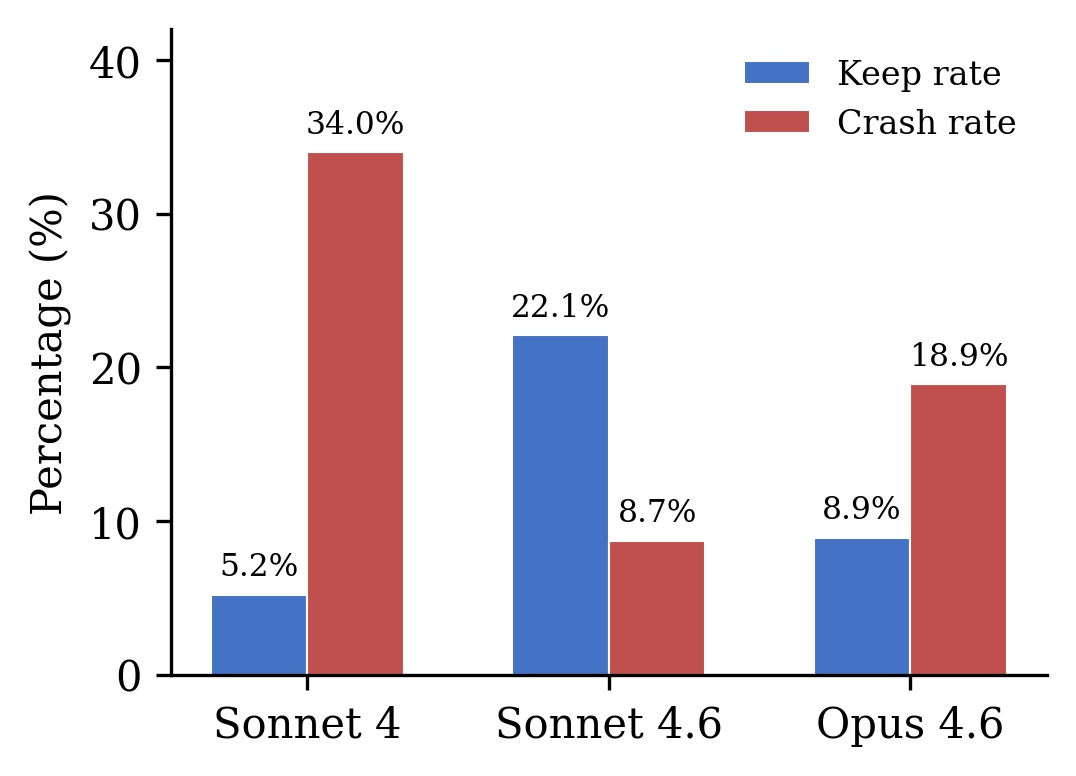
\includegraphics[width=0.7\textwidth]{figures/crash_rates.png}
\caption{Crash rates by model. Lower is better. Sonnet 4.6's low crash rate indicates the best understanding of code constraints among the three Phase 1 models.}
\label{fig:crash_rates}
\end{figure}

We categorize crashes into five types:

\begin{enumerate}[leftmargin=*]
    \item \textbf{Compilation failures}: Changes that break \texttt{torch.compile} graph tracing or cause GPU kernel launch errors. These include dynamic shapes, data-dependent branches, and unsupported operations.
    \item \textbf{Runtime errors}: Out-of-memory (OOM) from increased batch or model sizes, numerical instability (NaN losses), and dimension mismatches.
    \item \textbf{Inductor bugs}: Intermittent \texttt{torch.compile} backend failures unrelated to the proposed change.
    \item \textbf{Apply failed}: The LLM's proposed code patch could not be applied due to ambiguous or missing match targets.
    \item \textbf{Uncategorized}: Crashes where the error log was truncated, preventing automated classification.
\end{enumerate}

Table~\ref{tab:crash_categories} shows the breakdown of crash types by model.

\begin{table}[H]
\centering
\caption{Crash categorization by model, based on error log analysis. ``Compilation'' includes \texttt{torch.compile} graph tracing failures and GPU kernel launch errors. ``Apply failed'' means the LLM's proposed code patch could not be applied (ambiguous or missing match). ``Inductor'' refers to intermittent PyTorch inductor backend bugs unrelated to the proposed change.}
\label{tab:crash_categories}
\begin{tabular}{lrrr}
\toprule
\textbf{Crash Type} & \textbf{Sonnet 4} & \textbf{Sonnet 4.6} & \textbf{Opus 4.6} \\
\midrule
Compilation failure  & 15 (30\%) & 0 (0\%)   & 11 (52\%) \\
Runtime error        & 10 (20\%) & 1 (11\%)  & 1 (5\%)   \\
Inductor bug         & 3 (6\%)   & 1 (11\%)  & 1 (5\%)   \\
Apply failed         & 1 (2\%)   & 5 (56\%)  & 0 (0\%)   \\
Uncategorized        & 21 (42\%) & 2 (22\%)  & 8 (38\%)  \\
\midrule
Total                & 50        & 9         & 21        \\
\bottomrule
\end{tabular}
\end{table}

Compilation failures and uncategorized crashes dominate. The high ``uncategorized'' count reflects crashes where the error message was truncated in the TSV log, making automated classification difficult. Sonnet 4.6's crashes were predominantly failed code patches (the LLM proposed changes that could not be applied to the source), rather than training failures -- indicating conservative but imprecise code modification strategies.

% -----------------------------------------------------------------------------
\subsection{Cost-Effectiveness}
\label{sec:cost}
% -----------------------------------------------------------------------------

Table~\ref{tab:cost} presents cost-effectiveness metrics for each model.

\begin{table}[H]
\centering
\caption{Cost-effectiveness analysis. API cost is estimated from token usage. GPU cost assumes \$0.50/hr equivalent for electricity and amortization. Cost per 1\% improvement is the total cost divided by the percentage improvement achieved.}
\label{tab:cost}
\begin{tabular}{lrrr}
\toprule
\textbf{Metric} & \textbf{Sonnet 4} & \textbf{Sonnet 4.6} & \textbf{Opus 4.6} \\
\midrule
API cost (est.)      & \$8.82  & \$6.24  & \$50.00  \\
GPU time (hrs)       & 12.25   & 8.67    & 9.25     \\
GPU cost (est.)      & \$6.13  & \$4.33  & \$4.63   \\
Total cost (est.)    & \$14.95 & \$10.57 & \$54.63  \\
Improvement (\%)     & 1.25    & 23.24   & 5.64     \\
\textbf{Cost / 1\% impr.} & \textbf{\$11.96} & \textbf{\$0.45}  & \textbf{\$9.69}  \\
\bottomrule
\end{tabular}
\end{table}

Sonnet 4.6 is the clear efficiency winner at \$0.45 per 1\% improvement. However, this comparison is influenced by the baseline difference: Sonnet 4.6 started from the unoptimized master branch where improvements are easier to find. A fairer comparison would control for baseline difficulty, which we discuss in Section~\ref{sec:limitations}.

Opus 4.6's cost per 1\% improvement (\$9.69) appears expensive, but it operated on a much harder baseline. The absolute best val\_bpb of 0.9019 was only achievable through Opus 4.6's extended reasoning, making it cost-effective when measured against the final performance ceiling rather than percentage improvement.

% =============================================================================
\section{Phase 2: Controlled Head-to-Head Comparison (In Progress)}
\label{sec:phase2}
% =============================================================================

To address the baseline inconsistency identified in Phase 1, we designed a controlled experiment where all models start from an identical, unoptimized baseline.

% -----------------------------------------------------------------------------
\subsection{Experimental Design}
\label{sec:phase2_design}
% -----------------------------------------------------------------------------

The controlled comparison uses the following protocol:

\begin{enumerate}[leftmargin=*]
    \item \textbf{Frozen baseline.} We reset \texttt{train.py} to the upstream Karpathy defaults (Table~\ref{tab:phase2_baseline}), adding only the minimum hardware compatibility patches for Blackwell GPUs (SDPA attention fallback). No hyperparameter optimization is included.
    \item \textbf{Identical starting point.} All models branch from the same git commit (\texttt{3fb6704}), ensuring byte-identical starting code.
    \item \textbf{$n=3$ replication.} Each model runs three independent 100-experiment sessions. This enables computation of mean and standard deviation for keep rate, crash rate, and final val\_bpb, providing statistical confidence in the comparison.
    \item \textbf{Same hardware and dataset.} All runs use the RTX 5070 Ti with PubMed abstracts, matching Phase 1 conditions.
\end{enumerate}

\begin{table}[H]
\centering
\caption{Controlled baseline hyperparameters (upstream Karpathy defaults).}
\label{tab:phase2_baseline}
\begin{tabular}{ll}
\toprule
\textbf{Parameter} & \textbf{Value} \\
\midrule
WARMDOWN\_RATIO & 0.5 \\
MATRIX\_LR & 0.04 \\
WEIGHT\_DECAY & 0.2 \\
EMBEDDING\_LR & 0.6 \\
TOTAL\_BATCH\_SIZE & $2^{19}$ (524K tokens) \\
FINAL\_LR\_FRAC & 0.0 \\
Baseline val\_bpb & 1.097 \\
\bottomrule
\end{tabular}
\end{table}

The unoptimized baseline (val\_bpb = 1.097) provides substantial room for improvement. Known optimizations such as batch size reduction, warmdown ratio tuning, and per-group optimizer adjustments are all available for the models to discover independently.

% -----------------------------------------------------------------------------
\subsection{Run Schedule}
\label{sec:phase2_schedule}
% -----------------------------------------------------------------------------

Table~\ref{tab:phase2_runs} summarizes the planned runs. GPT-4.1 runs use Azure credits at zero marginal cost. Sonnet runs use the Anthropic API. Opus runs are the most expensive due to the 32K extended thinking budget.

\begin{table}[H]
\centering
\caption{Phase 2 controlled comparison: planned runs.}
\label{tab:phase2_runs}
\begin{tabular}{llllr}
\toprule
\textbf{Run} & \textbf{Model} & \textbf{API} & \textbf{Status} & \textbf{Est.\ Cost} \\
\midrule
1--3  & GPT-4.1           & Azure OpenAI & In progress & \$0 \\
4--6  & Claude Sonnet 4.6 & Anthropic    & Planned     & \$18 \\
7--9  & Claude Sonnet 4   & Anthropic    & Planned     & \$18 \\
10--12 & Claude Opus 4.6  & Anthropic    & Planned     & \$150 \\
\midrule
\multicolumn{4}{l}{\textbf{Total (12 runs $\times$ 100 experiments)}} & \textbf{\$186} \\
\bottomrule
\end{tabular}
\end{table}

% -----------------------------------------------------------------------------
\subsection{Expected Analyses}
\label{sec:phase2_analyses}
% -----------------------------------------------------------------------------

With $n=3$ runs per model, Phase 2 will enable:

\begin{itemize}[leftmargin=*]
    \item \textbf{Statistical comparison} of keep rates and crash rates with confidence intervals.
    \item \textbf{Reproducibility assessment} via variance across runs of the same model.
    \item \textbf{Learning curve analysis} comparing how quickly each model discovers key optimizations (e.g., batch size halving).
    \item \textbf{Strategy diversity analysis} comparing whether different runs of the same model discover the same or different optimization paths.
\end{itemize}

Phase 2 results will be reported in v2 of this manuscript.

% =============================================================================
\section{Discussion}
\label{sec:discussion}
% =============================================================================

% -----------------------------------------------------------------------------
\subsection{Model Capability Translates to Research Quality}
\label{sec:capability}
% -----------------------------------------------------------------------------

A clear hierarchy emerges from the results:

\begin{enumerate}[leftmargin=*]
    \item \textbf{Constraint awareness} (crash avoidance): Sonnet 4.6 $>$ Opus 4.6 $>$ Sonnet 4
    \item \textbf{Optimization efficiency} (keep rate): Sonnet 4.6 (22.1\%) $>$ Opus 4.6 (8.9\%) $>$ Sonnet 4 (5.2\%)
    \item \textbf{Depth of insight} (final val\_bpb): Opus 4.6 (0.9019) $>$ Sonnet 4 (0.9362) $>$ Sonnet 4.6 (0.9559)
\end{enumerate}

Constraint awareness -- the ability to learn from failed experiments and avoid repeating the same categories of errors -- appears to be the most differentiating factor for practical efficiency. Sonnet 4.6's low crash rate meant that almost every API call produced a meaningful result (either a kept improvement or an informative discard), while Sonnet 4 lost 34\% of its compute budget to crashes.

The depth-of-insight ranking differs from the efficiency ranking because Opus 4.6 operated on a harder baseline. This suggests that different models may be optimal for different phases of optimization: Sonnet 4.6 for rapid initial improvement, Opus 4.6 for squeezing out final gains.

% -----------------------------------------------------------------------------
\subsection{Extended Thinking for Hard Problems}
\label{sec:thinking}
% -----------------------------------------------------------------------------

The \texttt{grad\_accum=1} discovery chain (Section~\ref{sec:discoveries}) demonstrates why extended thinking matters. The reasoning required:

\begin{enumerate}[leftmargin=*]
    \item Recognizing that \texttt{grad\_accum=2} with batch size 32 means the optimizer updates every 64 samples.
    \item Reasoning that \texttt{grad\_accum=1} would double optimizer updates in the same wall-clock time.
    \item Predicting that doubled updates would effectively double weight decay application.
    \item Proposing halved weight decay to compensate.
    \item Further adjusting learning rates for the new update frequency.
\end{enumerate}

Each step depends on the previous one. Without extended thinking, the model would need to discover each compensation independently through trial and error, requiring multiple experiment rounds. With extended thinking, Opus 4.6 proposed steps 1--4 as a single coherent change, which succeeded on the first attempt.

This pattern -- multi-step causal reasoning about optimization dynamics -- is precisely the type of problem where extended thinking provides the most value. For simpler optimizations (batch size tuning, learning rate adjustments), the additional reasoning budget is unnecessary and the cost premium is not justified.

% -----------------------------------------------------------------------------
\subsection{Blackwell GPU Challenges}
\label{sec:blackwell}
% -----------------------------------------------------------------------------

Running \texttt{autoresearch} on an RTX 5070 Ti (Blackwell, SM 12.0) required solving several compatibility issues that may affect other researchers with new hardware:

\begin{enumerate}[leftmargin=*]
    \item \textbf{\texttt{torch.compile} inductor bugs.} Intermittent segmentation faults during compilation, unrelated to the code being compiled. Our auto-restart mechanism handled these transparently, but they add noise to experiment timings. We observed roughly 1 inductor crash per 30 experiments.
    \item \textbf{Jinja2 version sensitivity.} PyTorch 2.9.1 with CUDA 12.8 requires \texttt{jinja2 < 3.1.5} due to template rendering changes in the Triton backend. The symptom is a cryptic compilation error with no obvious connection to Jinja2.
    \item \textbf{Python version requirements.} Python 3.10's \texttt{sre\_parse} module has bugs triggered by certain regex patterns in the PyTorch codebase. Python 3.12 resolves these.
    \item \textbf{Flash Attention unavailability.} Flash Attention 3 \citep{dao2024flashattention3} had not been ported to Blackwell at the time of these experiments. SDPA provides the same functionality with slightly lower throughput.
\end{enumerate}

% -----------------------------------------------------------------------------
\subsection{Limitations}
\label{sec:limitations}
% -----------------------------------------------------------------------------

Several limitations constrain the generalizability of our findings:

\begin{enumerate}[leftmargin=*]
    \item \textbf{Single GPU, single dataset.} All experiments used one GPU configuration and one dataset. Results may differ on larger models, different hardware, or different text domains.
    \item \textbf{Hyperparameter-focused search.} Due to \texttt{torch.compile} fragility, the effective search space was dominated by numerical hyperparameter changes. Architecture search results might differ, particularly on frameworks that support dynamic modifications more gracefully.
    \item \textbf{val\_bpb as a proxy metric.} Bits-per-byte measures language modeling quality but does not directly measure downstream task performance (e.g., medical information extraction from PubMed abstracts).
    \item \textbf{Different baselines (Phase 1).} The sequential nature of Phase 1 experiments prevents apples-to-apples comparison. Phase 2 (Section~\ref{sec:phase2}) addresses this with a controlled identical-baseline design.
    \item \textbf{Single runs (Phase 1).} Each model was run once in Phase 1. Phase 2 uses $n=3$ runs per model to assess reproducibility and compute confidence intervals.
    \item \textbf{API pricing changes.} Cost estimates reflect pricing at the time of experiments (March 2026) and will likely change.
\end{enumerate}

% =============================================================================
\section{Practical Guide for Reproduction}
\label{sec:guide}
% =============================================================================

This section provides step-by-step instructions for researchers wishing to reproduce or extend our results. The \texttt{autoresearch} framework is available at \url{https://github.com/karpathy/autoresearch}.

% -----------------------------------------------------------------------------
\subsection{Hardware Requirements}
\label{sec:hw_requirements}
% -----------------------------------------------------------------------------

\begin{itemize}[leftmargin=*]
    \item \textbf{Minimum:} Any NVIDIA GPU with 12+ GB VRAM and CUDA 12.0+ support. The 50M-parameter model fits comfortably in 8GB, but training overhead requires additional headroom.
    \item \textbf{Recommended:} RTX 4070 Ti or newer. Older architectures (Ampere, Hopper) have more stable \texttt{torch.compile} support.
    \item \textbf{For Blackwell GPUs (50-series):} Expect intermittent inductor bugs. Ensure auto-restart is enabled in the framework.
\end{itemize}

% -----------------------------------------------------------------------------
\subsection{Environment Setup}
\label{sec:env_setup}
% -----------------------------------------------------------------------------

\begin{enumerate}[leftmargin=*]
    \item \textbf{Python 3.12+} is required. Do not use Python 3.10 (regex bugs) or 3.11 (untested).
    \item \textbf{Pin Jinja2:} \texttt{pip install "jinja2<3.1.5"} before installing PyTorch.
    \item \textbf{WSL2 recommended on Windows.} Native Windows PyTorch lacks full \texttt{torch.compile} support.
    \item \textbf{API keys:} Set \texttt{ANTHROPIC\_API\_KEY} for Claude models and configure Azure OpenAI endpoint for GPT-4.1.
\end{enumerate}

% -----------------------------------------------------------------------------
\subsection{Running Experiments}
\label{sec:running}
% -----------------------------------------------------------------------------

\begin{enumerate}[leftmargin=*]
    \item Clone the repository and install dependencies.
    \item Prepare the PubMed dataset: \texttt{python data/prepare\_pubmed.py}
    \item Run the baseline: \texttt{python train.py} (verify val\_bpb matches expected range).
    \item Launch autoresearch: \texttt{python autoresearch.py --model claude-sonnet-4.6 --experiments 100}
    \item Monitor via the Rich TUI dashboard showing real-time experiment status, val\_bpb history, and GPU metrics.
\end{enumerate}

% -----------------------------------------------------------------------------
\subsection{Common Pitfalls}
\label{sec:pitfalls}
% -----------------------------------------------------------------------------

\begin{itemize}[leftmargin=*]
    \item \textbf{GPU thermal throttling.} Consumer GPUs without adequate cooling will thermal-throttle during sustained training. Monitor temperatures. Our framework pauses at 80\textdegree C and aborts at 90\textdegree C to prevent hardware damage.
    \item \textbf{API billing surprises.} Opus 4.6 with extended thinking can cost \$1--2 per experiment. Budget \$50--100 for a 100-experiment Opus run. Set billing alerts.
    \item \textbf{Disk space.} Experiment logs and model checkpoints accumulate. Expect 5--10 GB per 100-experiment run.
    \item \textbf{\texttt{torch.compile} cache.} The compilation cache can grow large and occasionally become corrupted. Clear it (\texttt{rm -rf \~{}/.cache/torch/inductor}) if experiments show unexplained compilation failures.
\end{itemize}

% -----------------------------------------------------------------------------
\subsection{Cost Planning}
\label{sec:cost_planning}
% -----------------------------------------------------------------------------

Table~\ref{tab:budget} provides budget estimates for various experiment scales.

\begin{table}[H]
\centering
\caption{Estimated costs for different experiment configurations (API costs only, March 2026 pricing).}
\label{tab:budget}
\begin{tabular}{lrrr}
\toprule
\textbf{Model} & \textbf{50 Experiments} & \textbf{100 Experiments} & \textbf{200 Experiments} \\
\midrule
Sonnet 4 / 4.6 & \$3 & \$6 & \$12  \\
Opus 4.6 (32K thinking) & \$50--100 & \$100--200 & \$200--400 \\
\bottomrule
\end{tabular}
\end{table}

Our recommendation: start with 100 experiments of Sonnet 4.6 to establish a strong baseline (\textasciitilde\$6 API cost), then run 50--100 experiments of Opus 4.6 on the optimized result if further improvement is desired (\textasciitilde\$50--100 API cost).

% =============================================================================
\section{Conclusion}
\label{sec:conclusion}
% =============================================================================

We presented an experimental comparison of LLMs as autonomous ML researchers, evaluating three models in Phase 1 on the task of optimizing a 50M-parameter language model's training configuration. While Phase 1's sequential design limits direct comparison (addressed by the controlled Phase 2), several findings emerge:

\begin{enumerate}[leftmargin=*]
    \item \textbf{LLM capability directly impacts autonomous research quality.} Crash rates, keep rates, and the depth of discovered optimizations all correlate with model capability. The gap between the best (Sonnet 4.6) and worst (Sonnet 4) Phase 1 performers is substantial.

    \item \textbf{Sonnet 4.6 is the efficiency optimum for most researchers.} With the highest keep rate (22.1\%), lowest crash rate (8.7\%), and best cost-effectiveness (\$0.45 per 1\% improvement), Sonnet 4.6 is the recommended starting point for autonomous optimization experiments.

    \item \textbf{Extended thinking enables deeper optimization.} Opus 4.6 found multi-step optimization chains that other models could not, achieving the best absolute val\_bpb (0.9019) on an already-optimized baseline. The cost premium is justified when the baseline is already strong and incremental improvements require causal reasoning about optimizer dynamics.

    \item \textbf{Open-source tooling makes this accessible.} The \texttt{autoresearch} framework, combined with consumer-grade GPUs and standard API access, enables any researcher to run autonomous optimization experiments. The total cost for a comprehensive 100-experiment run with Sonnet 4.6 is under \$11 including GPU electricity.
\end{enumerate}

Phase 2 of this study (Section~\ref{sec:phase2}), currently in progress, directly addresses the two primary limitations: baseline inconsistency and single-run variance. Preliminary Phase 2 results for GPT-4.1 are being collected at time of writing. Additional future work should explore multi-GPU scaling, architecture search with more flexible compilation frameworks, evaluation on downstream tasks rather than proxy metrics, and cross-hardware validation with collaborator-contributed results.

These results suggest that LLMs are becoming practically useful for the specific subtask of iterative training optimization. They cannot formulate novel research questions, contextualize results in the broader scientific landscape, or reason about which experiments are worth running. But within a well-defined optimization loop with clear metrics, they can discover meaningful improvements autonomously. The degree to which this generalizes beyond hyperparameter tuning to broader research tasks remains an open question.

% =============================================================================
\section*{Acknowledgments}
\label{sec:acknowledgments}
% =============================================================================

We thank Andrej Karpathy for creating the \texttt{autoresearch} framework and for the broader vision of autonomous ML research that inspired this work.

We thank the open-source community whose tools made this work possible: the PyTorch team for \texttt{torch.compile} and the broader framework; the Triton team for GPU kernel compilation; Hugging Face for dataset hosting and the Transformers ecosystem; and Will McGugan and the Textualize team for the Rich TUI library used in experiment monitoring.

We thank Anthropic for API access to Claude Sonnet 4, Claude Sonnet 4.6, and Claude Opus 4.6, and for technical support during the extended thinking integration.

We thank Microsoft Azure and OpenAI for GPT-4.1 API access.

We gratefully acknowledge Renato Umeton, Ph.D., for guidance on publication and for championing open-source contributions to the ML research community.

We thank Dave Graham from ML Commons for working alongside us, sharing insights from his parallel research efforts, and for the accountability and motivation that made the overnight experiment runs possible.

We thank the LinkedIn ML/NLP community for feedback, discussion, and interest in early results shared during the course of this research.

% =============================================================================
% References
% =============================================================================
\bibliographystyle{plainnat}

\begin{thebibliography}{11}

\bibitem[Chen et~al.(2021)]{chen2021codex}
M.~Chen, J.~Tworek, H.~Jun, Q.~Yuan, H.~Pinto de~Oliveira, J.~Kaplan, H.~Edwards, Y.~Burda, N.~Joseph, G.~Brockman, A.~Ray, R.~Puri, G.~Krueger, M.~Petrov, H.~Khlaaf, G.~Sastry, P.~Mishkin, B.~Chan, S.~Gray, N.~Ryder, M.~Pavlov, A.~Power, L.~Kaiser, M.~Bavarian, C.~Winter, P.~Tillet, F.~P. Such, D.~Cummings, M.~Plappert, F.~Chantzis, E.~Barnes, A.~Herbert-Voss, W.~H. Guss, A.~Nichol, A.~Paino, N.~Tezak, J.~Tang, I.~Babuschkin, S.~Balaji, S.~Jain, W.~Saunders, C.~Hesse, A.~N. Carr, J.~Leike, J.~Achiam, V.~Misra, E.~Morikawa, A.~Radford, M.~Knight, M.~Brundage, M.~Murati, K.~Mayer, P.~Welinder, B.~McGrew, D.~Amodei, S.~McCandlish, I.~Sutskever, and W.~Zaremba.
\newblock Evaluating large language models trained on code.
\newblock \emph{arXiv preprint arXiv:2107.03374}, 2021.

\bibitem[Dao(2024)]{dao2024flashattention3}
T.~Dao.
\newblock {FlashAttention-3}: Fast and exact attention with asymmetric attention.
\newblock \emph{arXiv preprint}, 2024.

\bibitem[Hutter et~al.(2019)]{hutter2019automl}
F.~Hutter, L.~Kotthoff, and J.~Vanschoren, editors.
\newblock \emph{Automated Machine Learning: Methods, Systems, Challenges}.
\newblock Springer, 2019.


\bibitem[Karpathy(2026)]{karpathy2026autoresearch}
A.~Karpathy.
\newblock autoresearch.
\newblock \url{https://github.com/karpathy/autoresearch}, 2026.

\bibitem[Lu et~al.(2024)]{lu2024aiscientist}
C.~Lu, C.~Lu, R.~T. Lange, J.~Foerster, J.~Clune, and D.~Ha.
\newblock The {AI} {Scientist}: Towards fully automated open-ended scientific discovery.
\newblock \emph{arXiv preprint arXiv:2408.06292}, 2024.

\bibitem[{OpenAI}(2025)]{openai2025gpt41}
{OpenAI}.
\newblock {GPT-4.1}.
\newblock \url{https://platform.openai.com}, 2025.

\bibitem[{Anthropic}(2026)]{anthropic2026claude}
{Anthropic}.
\newblock {Claude Sonnet 4.6 and Opus 4.6}.
\newblock \url{https://www.anthropic.com}, 2026.

\bibitem[{PyTorch Team}(2024)]{pytorch2024compile}
{PyTorch Team}.
\newblock \texttt{torch.compile}: Making {PyTorch} code faster.
\newblock \url{https://pytorch.org/docs/stable/torch.compiler.html}, 2024.

\bibitem[Jordan et~al.(2024)]{jordan2024muon}
K.~Jordan, Y.~Jin, V.~Boza, J.~You, F.~Cesista, L.~Newhouse, and J.~Bernstein.
\newblock Muon: An optimizer for hidden layers in neural networks.
\newblock \url{https://kellerjordan.github.io/posts/muon/}, 2024.

\bibitem[Zoph and Le(2017)]{zoph2017nas}
B.~Zoph and Q.~V. Le.
\newblock Neural architecture search with reinforcement learning.
\newblock In \emph{International Conference on Learning Representations ({ICLR})}, 2017.

\end{thebibliography}

\end{document}
